\documentclass{bioinfo}
\copyrightyear{2017} \pubyear{2017}

\access{Advance Access Publication Date: Day Month Year}
\appnotes{Application Note}

\usepackage{url}

\begin{document}
\firstpage{1}

\subtitle{Subject Section}

\title[short Title]{Phylotyper: In silico predictor of bacterial subtypes from gene sequences}
\author[Whiteside \textit{et~al}.]{Matthew D. Whiteside\,$^{\text{\sfb 1,}*}$, Chad R. Laing\,$^{\text{\sfb 1}}$ and Victor P.J. Gannon\,$^{\text{\sfb 1,}*}$}
\address{$^{\text{\sf 1}}$National Microbiology Laboratory, Public Health Agency of Canada, Lethbridge, AB, Canada, T1J 3Z4}

\corresp{$^\ast$To whom correspondence should be addressed.}

\history{Received on XXXXX; revised on XXXXX; accepted on XXXXX}

\editor{Associate Editor: XXXXXXX}

\abstract{\textbf{Motivation:} Text Text Text Text Text Text Text Text Text Text Text Text Text
Text Text Text Text Text Text Text Text Text Text Text Text Text Text Text Text Text Text Text
Text Text Text Text Text Text Text Text Text Text Text Text Text Text Text Text Text Text Text
Text Text Text Text Text Text
Text Text Text Text Text.\\
\textbf{Results:} Text  Text Text Text Text Text Text Text Text Text  Text Text Text Text Text
Text Text Text Text Text Text Text Text Text Text Text Text Text  Text Text Text Text Text Text\\
\textbf{Availability:} Phylotyper is available for download from: \url{https://github.com/superphy/insilico-subtyping}.\\
\textbf{Contact:} \href{matthew.whiteside@phac-aspc.gc.ca}{matthew.whiteside@phac-aspc.gc.ca}\\
\textbf{Supplementary information:} Supplementary data are available at \textit{Bioinformatics}
online.}

\maketitle

\section{Introduction}

http://genomemedicine.biomedcentral.com/articles/10.1186/s13073-014-0090-6

https://holtlab.net/2014/12/27/behind-the-paper-srst2-for-short-read-sequence-typing-of-bacterial-pathogens/

http://jcm.asm.org/content/53/8/2410.full

http://mgen.microbiologyresearch.org/content/journal/mgen/10.1099/mgen.0.000064

https://www.ncbi.nlm.nih.gov/pmc/articles/PMC4876609/

https://www.ncbi.nlm.nih.gov/pmc/articles/PMC4508412/

Whole-genome sequencing (WGS) is a transformative technology.
In public health, the speed, discriminatory power and broad utility of WGS data promises to improve surviellence and outbreak analysis.
Adoption of WGS in the public health, however, requires bridging of historical data and systems with new the technologies and data.
One of the workhorse methods used in public health are phenotypic subtyping (such as serotyping).
As a survillence tool, subtypes provide an straight-forward designation that is typically used to distinguish taxonomic groups and infer phenotypes, for example, pathogens from non-pathogens.
A WGS-based approach to subtyping would have several benefits over current subtype systems; improved discrimination, cheaper and easier to maintain and routinely run, and would be faster.
Accordingly, new \textit{in silico} tools have been developed to predict subtypes from WGS data.

The current \textit{in silico} predictors of bacterial subtypes use a similar approach; genes or genome sequences with unknown type are compared against a reference database of sequences with known subtypes.
Subtype assignment is based on sequence similarity with the subtype annotation from the top match above a pre-selected sequence similarity threshold being used to assign a subtype to the unknown query.
These tools do not examine the phylogenetic context or consider rate of sequence mutation within and between subtypes.
Sequence similarity scores are not direct indicators of the level of uncertainty assocated with a subtype prediction.

Phylotyper is a novel in silico predictor of subtypes from sequence data. 
It builds a phylogenetic tree consisting of reference sequences with known subtype and the unknown query sequences.  
Using phylogenetic ancestral reconstruction to assign likelihoods of each type to the branch points in the tree and also compute the transition rates between subtypes, Phylotyper assigns an unknown query sequence a subtype based on the extrapolated value from its ancestors in the tree.
Subtype information is mainly used as a proxy for evolutionarily-related bacterial strain groups or to infer phenotypes.
A phylogenetic framework for predicting subtypes is more consistent with the main uses of subtype information.


\section{The Phylotyper Approach}

The core of Phylotyper, is an ancestral state reconstruction method that has been adapted for hidden state prediction.
In phylogenetics, ancestral state reconstruction involves the prediction of traits of ancestors from extant descendants.
This methodology can be extended to predict properties in existing strains under investigation for which the a properties' state is unknown.
Ancestral state reconstruction (ASR) has been successfully applied to hidden state prediction in the field of microbial metagenomics; the tool PICRUSt uses ASR to estimate the gene family content contributed by a bacteria to a metagenomic sample.

In Phylotyper, the \texttt{rerootingMethod} function from the phytools R package is used to perform the ASR.
It is based on a method originally described in Yang \emph{et al}. (1995) for estimating the marginal likelihood of a discrete set of states for the internal nodes in a phylogenetic tree.
The phytools \texttt{rerootingMethod} function was selected over alternatives, such as APE ace, because it can handle extant tip nodes with unkown states in the phylogenetic tree and also compute posterior probability for those nodes, hence, making applicable for hidden state prediction.
The maximum marginal likelihood (also called emperical Bayesian posterior probability) calculated for unknown tip nodes reflects the most likely state for the node given the emperically estimated evolution model and phylogeny.
It captures the uncertainty associated with phylogenetic branch lengths and rates of change associated with the states.
In the context of Phylotyper, the posterior probabilities provides a confidence value associated with a predicted subtype.
The evolutionary model used in \texttt{rerootingMethod} is the $\text{M}_{\text{k}}$ model for discrete states (a continuous-time Markov process model)).  
It is estimated from the data, so in Phylotyper, the reference set of genes used to build a phylogenetic tree and run the ASR, is key to the performance of the predictor.
For subtype schemes packaged in Phylotyper, the annotated genes will be maintained and routinely updated to provide a robust and comprehensive reference set.
The other key assumption is that gene phylogeny is correlated with the evolution of subtype state.
Because of these assumptions are central to the method, all new subtype schemes added into Phylotyper are evaluated for their predictive performance.

Phylotyper is developed in python and R. 
Outlined below are the steps and tools used in the Phylotyper pipeline:

\begin{enumerate}
\item Identify subtype gene loci in input genomes using blastn or blastx.
\item Align input genes with unknown sunbtype against a pre-aligned set of reference genes using the tool MAFFT's \texttt{--add} feature.
\item If multiple loci are involved, concatenate individual alignments into superalignment.
\item Generate phylogenetic tree of aligned genes with FastTree.
\item Run phytools \texttt{rerootingMethod} using the phylogenetic tree and assigned subtypes. 
Genes with unknown subtype are assigned a flat prior.
\item Identify the subtype with maximum marginal likelihood for the unknown genes and report to user.
Users are also provided with a image of the phylogenetic tree that shows the position of the unknown genes. 
An example is shown in Figure~1\vphantom{\ref{fig:01}}.
\end{enumerate}

\section{Functionality in the Phylotyper Tool}

Phylotyper was designed to be incorporated into a whole genome sequencing public health workflow.  
The main input into Phylotyper is assembled (but not necessarily closed) genome sequences.  
Putative loci needed for the selected subtype scheme are identified in the input genomes using BLAST.
The discovered loci are then sent to the Phylotyper subtype prediction module.
It is possible to bypass the loci search step and provide genes directly to Phylotyper using the subtype run mode.

The Phylotyper approach can be used to predict any biological property that can be inferred from the phylogenetic distribution of a nominal set of genomic loci.
Currently, subtype schemes for \emph{Escherichia coli} Shiga-toxin 1 and 2 subtypes, Serotype O and H-types and Intimin subtypes are available in the Phylotyper package.
Details about the current schemes available in the Phylotyper package is provided in table XXX.
However, included in the Phylotyper software, is the capability to add new subtype schemes. 
Creating a new subtype scheme will save the required reference files in a data directory, allowing the newly added schemes to be easily run from Phylotyper. 
We also encourage users to contribute their subtype schemes to the main software repository (please send us subtype schemes you have developed and wish to share).

Checks are built-in new subtype scheme pipeline to ensure the main assumptions of the Phylotyper approach are not violated.  
A scan of the reference phylogenetic tree is conducted to search for tightly clustered subclades in the tree that have divergent subtypes.
We first estimate the distribution of the inter-patristic distances of genes with the same subtype.  
The distribution is used to dynamically select a distance threshold, which we employ to flag subclades wherein the inter-patristic distance is less than  the threshold but contains multiple distinct subtypes.
We also conduct a leave-one-out cross validation for each gene in the new subtype scheme to assess the scheme's predictive capability.
Users are alerted if their subtype schemes that have a F1-score below 0.9 from the cross-validation analysis.

Phylotyper also offers flexibility in the parameterization of evolution model used in the ASR step.
A component of the underlying ASR framework, is an Mk or markov model of subtype evolution, for which an emperical transition rate matrix is estimated from the data.
The transition matrix is used to calculate the expected number of subtype state changes given a distance in the phylogenetic tree.  
Different model parameterizations can be defined for the transition rate matrix. 
The simplest parameterization available in Phylotyper is the equal rates model; all subtypes have the same forward and reverse rate.  
The most complex parameterization available im Phylotyper is the symmetric model, wherein each forward and reverse rate for a given pair of subtypes are assigned a separate parameter.
Frequently, the number of subtypes makes the symmetric model too computationally prohibitive.
To offer more flexible models in these situations with reduced numbers of free parameters, two custom parameterization approaches were developed.
The custom approaches both use a binning strategy that attempts to identify sets of subtypes that would have similar rates and assign them a single parameter as a set.
These approaches are described in detail in the Supplementary Information XXX.
Each of these model parameterizations; equal, symmetric and the two custom models are tested and evaluated in new subtype pipeline.
The parameterization that has highest accuracy (based on a LOOCV analysis) is selected.
In the case of ties, the model with the fewest parameters is given precidence (the symmetric model is not tested when the number of subtypes is over 10)

In testing the predictive capability of Phylotyper, we found that in some cases, jointly using multiple loci increased the subtype prediction accuracy.  
And so, in Phylotyper, multiple loci can be used in creating subtype schemes.
The loci will be independently identified in the genome using BLAST and then independently aligned.  
The individual loci alignments are then concatenated to form a single superalignment that is used to build the predictive phylogenetic tree.  
The Stx1 and Stx2 schemes are examples of a multi-loci subtype schemes.  
The A and B subunit genes that make up the holo-toxin in Shiga-toxin are the inputs in these subtype schemes.


\section{Comparison to a Sequence Similarity Approach}

To assess the performance of the phylogenetic-based method used in Phylotyper and compare it to a direct sequence similarity-based approach, we ran a leave-one-out cross validation analysis. 
Each reference gene with experimentally validated subtype was removed from the training dataset and used as a test input into the Phylotyper program. 
Similarily, using a mock sequence-similarity based tool we developed for assessment purposes, each gene was witheld from the BLAST reference database and used as input (Source code is available in TODO).
The sequence-similarity tool assigns putative subtypes using a BLAST sequence search.  
The predicted subtype annotation for the test input is assigned from top BLAST hit, provided the top hit passes a percent identity, e-value and alignment coverage minimum thresholds.  
The threshold values are listed in TODO.
This approach of transfering annotations from genes with highest sequence similarity is the core of most current subtying methods.


\section{Discussion}

Phylotyper can...
New subtypes,
Performance test highly accurate.

Sequence does not develop a model of subtype evolution. 
Subtypes can evolve and different rates. 
Strict one-size fits all cutoffs will not work.  
The phylogenetic framework provides natural statistical interpretation of confidence values.



%%%%%%%%%%%%%%%%%%%%%%%%%%%%%%%%%%%%%%%%%%%%%%%%%%%%%%%%%%%%%%%%%%%%%%%%%%%%%%%%%%%%%
%
%     please remove the " % " symbol from \centerline{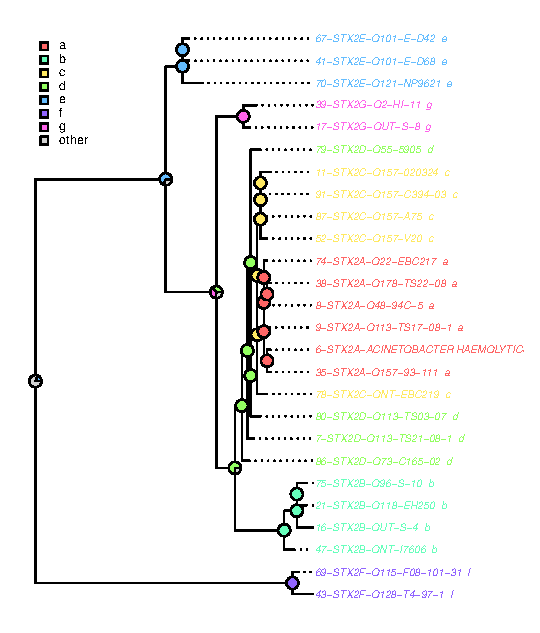
\includegraphics{fig01.eps}}
%     as it may ignore the figures.
%
%%%%%%%%%%%%%%%%%%%%%%%%%%%%%%%%%%%%%%%%%%%%%%%%%%%%%%%%%%%%%%%%%%%%%%%%%%%%%%%%%%%%%%


\section{Conclusion}

Text Text text\vspace*{-10pt}


\section*{Acknowledgements}

text text text\vspace*{-12pt}


\section*{Funding}

This work has been supported by the... \vspace*{-12pt}

%\bibliographystyle{natbib}
%\bibliographystyle{achemnat}
%\bibliographystyle{plainnat}
%\bibliographystyle{abbrv}
%\bibliographystyle{bioinformatics}
%
%\bibliographystyle{plain}
%
%\bibliography{Document}


\begin{thebibliography}{}

\bibitem[Bofelli {\it et~al}., 2000]{Boffelli03}
Bofelli,F., Name2, Name3 (2003) Article title, {\it Journal Name}, {\bf 199}, 133-154.

\bibitem[Bag {\it et~al}., 2001]{Bag01}
Bag,M., Name2, Name3 (2001) Article title, {\it Journal Name}, {\bf 99}, 33-54.

\bibitem[Yoo \textit{et~al}., 2003]{Yoo03}
Yoo,M.S. \textit{et~al}. (2003) Oxidative stress regulated genes
in nigral dopaminergic neurnol cell: correlation with the known
pathology in Parkinson's disease. \textit{Brain Res. Mol. Brain
Res.}, \textbf{110}(Suppl. 1), 76--84.

\bibitem[Lehmann, 1986]{Leh86}
Lehmann,E.L. (1986) Chapter title. \textit{Book Title}. Vol.~1, 2nd edn. Springer-Verlag, New York.

\bibitem[Crenshaw and Jones, 2003]{Cre03}
Crenshaw, B.,III, and Jones, W.B.,Jr (2003) The future of clinical
cancer management: one tumor, one chip. \textit{Bioinformatics},
doi:10.1093/bioinformatics/btn000.

\bibitem[Auhtor \textit{et~al}. (2000)]{Aut00}
Auhtor,A.B. \textit{et~al}. (2000) Chapter title. In Smith, A.C.
(ed.), \textit{Book Title}, 2nd edn. Publisher, Location, Vol. 1, pp.
???--???.

\bibitem[Bardet, 1920]{Bar20}
Bardet, G. (1920) Sur un syndrome d'obesite infantile avec
polydactylie et retinite pigmentaire (contribution a l'etude des
formes cliniques de l'obesite hypophysaire). PhD Thesis, name of
institution, Paris, France.

\end{thebibliography}
\end{document}
